\documentclass[uplatex,dvipdfmx,a4paper,10pt]{jsarticle}

\usepackage{amsmath,amsthm,amssymb}
\usepackage[dvipdfmx]{graphicx}
\usepackage{bm}
\usepackage{ascmac}
%
\usepackage{multirow}
\usepackage{wrapfig}
%
\pagestyle{empty}
%% 高さの設定
\usepackage{geometry}
\geometry{left=25truemm, right=25truemm, top=25truemm, bottom=25truemm}

%
\abovecaptionskip=-1pt
%\belowcaptionskip=-1pt
%
\renewcommand{\baselinestretch}{0.9} % 全体の行間調整
\renewcommand{\figurename}{Fig.}
\renewcommand{\tablename}{Tab.}
%
\makeatletter 
\def\section{\@startsection {section}{1}{\z@}{1.5 ex plus 2ex minus -.2ex}{0.5 ex plus .2ex}{\large\bf}}
\def\subsection{\@startsection{subsection}{2}{\z@}{0.2\Cvs \@plus.5\Cdp \@minus.2\Cdp}{0.1\Cvs \@plus.3\Cdp}{\reset@font\normalsize\bfseries}}
\makeatother 
%
\graphicspath{{../../figures//}}
%
\begin{document}

%%%%%%
% はじめに
%%%%%%
\begin{center}
{\Large \textgt{22. ランダム構造を有するネットワークポリマーの緩和挙動}}
\end{center}

\begin{flushright}
東亞合成 佐々木裕

Tel: 052-611-9923, e-mail: hiroshi\_sasaki$@$mail.toagosei.co.jp
\end{flushright}

\vspace{0.5\baselineskip}
\section{はじめに}

ゴムの大きな破壊靭性の由来については、 ヒステリシスロスのようなエネルギー散逸により亀裂進展が抑制されるという Andrews モデルが提案されている~\cite{Andrews1977}。
ゴムへのフィラーの添加がヒステリシスの主要な発生原因とされ~\cite{Grosch1968}、その発現機構の一つとしてフィラー近傍でのナノキャビティーの開閉も報告されている~\cite{Zhang2013}。
フィラー由来の靭性向上効果はメゾスケール領域の挙動であると考えられているが、このようなエネルギー散逸挙動はメゾスケールでしか発現しないのであろうか?

\section{シミュレーション}

\subsection{ネットワークモデルの作成}

任意の分岐数$f$($f=3\sim6$)の結節点からなる規則構造を有するネットワークに対して、トポロジーモデルの「代数的連結性」を指標として以下のアルゴリズムでランダムな結合性を導入した。
% \vspace{-2mm}
\begin{enumerate}
\item
実空間で"8-Strand Unit Cell"の周期境界での連なり(2x2x2=8 Cells)の初期構造を作成(Fig. \ref{fig:cells})。
\item
初期構造に対応したトポロジーモデルを用いてノードごとのエッジ数(分岐数)に変換(Fig. \ref{fig:topo})。
\item
トポロジーモデルにて、ネットワークの結びつきの強さを表す代数的連結性を指標として連結性を維持しながらストランド交換し、結節点の結合性にランダム性を導入(Fig. \ref{fig:exc})。
\item
そのトポロジーモデルに対応するように、実空間の初期構造からストランドを除去。
\end{enumerate}

\subsection{MD シミュレーション}

上記にて生成したランダムな結合性を有するネットワークを初期構造として、OCTA 上の COGNAC シミュレーターにより MD シミュレーションを行った。
ユニットセル中でのストランドの末端間距離がホモポリマーと同等になるようにストランド長と多重度を調整し、緩和計算により平衡構造を得た。

\begin{figure}[hb]
\begin{minipage}{0.34\hsize}
    \begin{center}
        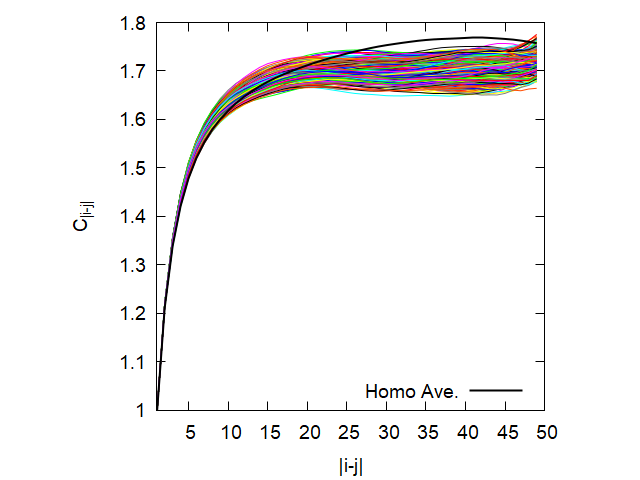
\includegraphics[width=\textwidth]{N48_f4_CN.png}
	    \caption{Trajectry of Mean Square Internal Distance distribution of strands for 4-Chain Model}
	    \label{fig:e2e}
	\end{center}
\end{minipage}
\begin{minipage}{0.34\hsize}
	\begin{center}
		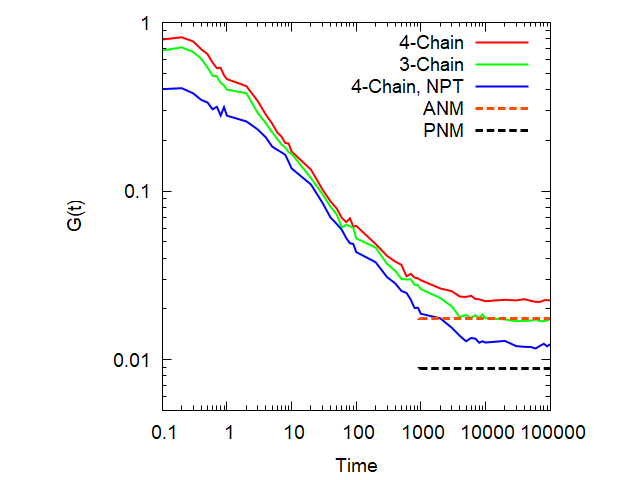
\includegraphics[width=\textwidth]{gt_comp_34.png}
        \caption{Stress Relaxations for Uni-axial Step Strain($\lambda=2$)}
        \label{fig:stress_rel}
	\end{center}
\end{minipage}
\begin{minipage}{0.32\hsize}
	\begin{center}
		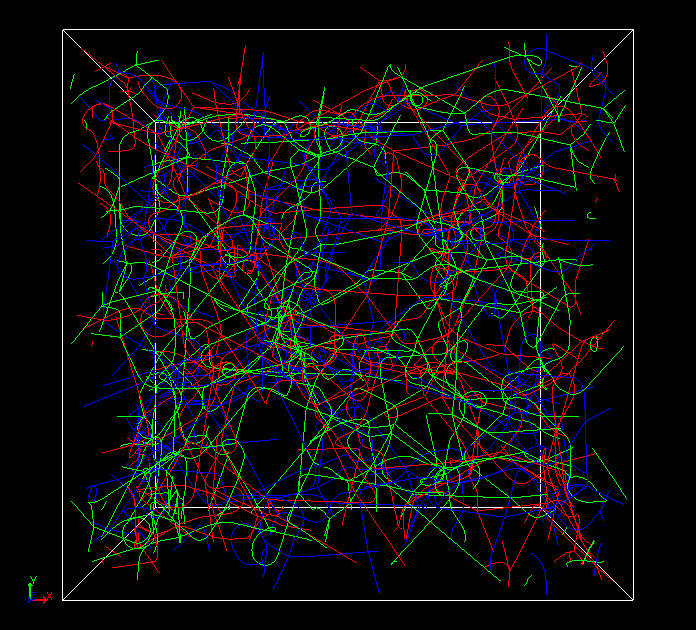
\includegraphics[width=.8\textwidth]{N48_f4_PPA.png}
        \caption{Primitive Path Analysis (PPA) for 4-Chain Model}
        \label{fig:ppa}
	\end{center}
\end{minipage}
\end{figure}

\vspace{-3mm}

\bibliographystyle{../achemso}
\bibliography{D:/Dropbox/Bibliography/library.bib}

\end{document}